\chapter{NAO Kinematics: The Solution}
\label{approach}

As mentioned in Chapter~\ref{related}, the existing approaches to kinematics for the NAO robot are not completely suitable for our needs. We seek to find a solution to the forward kinematics problem for any set of joint values as input and not only for the current joint values. In addition, we seek to find a real-time analytical solution for the problem of inverse kinematics without any approximations. In the sections below, we describe our solutions to both of these problems.


\section{Forward Kinematics for the NAO Robot}


Aldebaran Robotics provides the DH parameters for each kinematic chain of the robot in the documentation~\cite{AldebaranNaoDoc}. However, our experimentation with the provided values revealed that the given parameters for the arm chains are incorrect. Therefore, we found our own parameters for the arms and we used the provided parameters for the legs and the head.


\subsubsection*{NAO Zero Position}
We must define the base frame of the robot and the zero position of the joints before we proceed. The base frame is taken to be the torso frame; Figure~\ref{fig:torso} shows the axes of this frame. The same figure shows also the zero position of all the joints of the robot, which is the one provided by Aldebaran Robotics. As we can see, in this position the ShoulderRoll joints are not really roll joints, but are yaw joints, so we can understand that the names of the joints do not necessarily describe the actual movement of the joint in the base frame given the zero position.

\begin{figure}[h]
\begin{center}
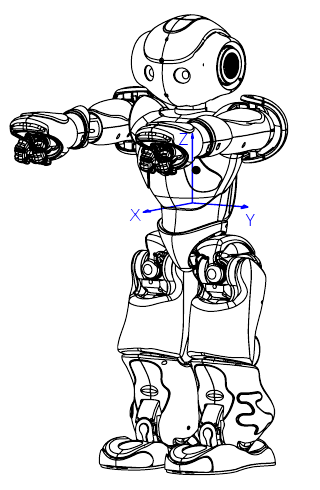
\includegraphics[height = 10cm]{Figures/torso_frame.png}
\caption{Base (torso) frame and zero position of the joints}
\label{fig:torso}
\end{center}
\end{figure}


\subsubsection*{Notation}
We provide a brief description of the symbols we use in our math calculations. All matrices used are affine transformation matrices of three types: $T$ is a transformation matrix, $R_x, R_y, R_z$ are basic rotations matrices, and $A$ is a translation matrix. The subscript of a symbol refers to the start frame and the superscript refers to the destination frame. The torso is the point where all the kinematic chains begin and is located at the center of the NAO body. ``Base'' is the start frame of the chain (the torso frame), while ``End'' is the end effector of the chain. The numbers appearing as subscripts or superscripts refer to the joints in the current kinematic chain, numbered consistently with the ordering given in the tables of Chapter~\ref{problem}. Also, we denote the initialization of a translation matrix as $A(d_x,d_y,d_z)$ and of rotation matrices as $R_x(\theta_x)$, $R_y(\theta_y)$, or $R_z(\theta_z)$.

We present the DH parameters of each kinematic chain in a separate table and, besides the DH parameters, we provide the translations from the ``Base'' to the first joint and from the last joint to the ``End''. Finally, we provide some necessary rotations to adjust the frame of the last joint to the frame of the end effector (``End'').


\subsubsection*{Forward Kinematics Equations}
Forward kinematics for each chain of the NAO robot is a transformation that maps a point from the frame of the last joint to the base frame. In our case, the end effector is the point of interest. Forward kinematics are defined in terms of transformation, rotation, and translation matrices, and the final result is a single transformation matrix that maps points from one frame to another. 

\subsubsection*{Extracting the Point in the Three-Dimensional Space}
The result of forward kinematics is an affine transformation matrix $T$ with the $X$ block being a rotation matrix and the $Y$ block being a translation vector. We need to extract the $(p_x, p_y, p_z)$ position and the $(a_x,a_y,a_z)$ orientations of the final point. The position $(p_x, p_y, p_z)$ can be simply read off the translation part of the transformation matrix:
\begin{align*}
p_x &= T_{(1,4)}\\
p_y &= T_{(2,4)}\\
p_z &= T_{(3,4)}
\end{align*}
The rotation of the final transformation table is a $R_zR_yR_x$ rotation table, whose analytical form is shown in Section~\ref{sec:affine}. Now it's easy to extract the orientation $(a_x,a_y,a_z)$:
\begin{align*}
a_x &= \arctan\!2 \left(T_{(3,2)},T_{(3,3)}\right)\\
a_y &= \arctan\!2 \left(-T_{(3,1)},\sqrt{{T_{(3,2)}}^2 + {T_{(3,3)}}^2}\right)\\
a_z &= \arctan\!2 \left(T_{(2,1)},T_{(1,1)}\right)
\end{align*}

\subsection{Forward Kinematics for the Head}
The head is the simplest kinematic chain of the NAO robot, but it has two useful end effectors, namely the top and the bottom cameras. Table~\ref{tab:DHhead} shows the DH parameters for the head chain. Now, we can combine these matrices to find the point of the end effector in the frame space of the torso:
\[
T^\text{End}_\text{Base} = A^0_\text{Base}T^1_0T^2_1R_x(\tfrac{\pi}{2})R_y(\tfrac{\pi}{2})A^\text{End}_{2}
\]
$T^1_0$ and $T^2_1$ are the DH transformation matrices of the corresponding joints (HeadYaw, HeadPitch). $A^\text{End}_{2}$ is one of the two translation matrices given in Table~\ref{tab:DHhead} for the two end effectors (top and bottom camera). The point of the end effector in the three-dimensional space of the torso can be extracted from $T^\text{End}_\text{Base}$.


\begin{table}[t!]
\centering
\caption{DH parameters for the Head chain}
\begin{tabular}{|l|>{\centering\arraybackslash}m{2.55cm}|>{\centering\arraybackslash}m{2.55cm}|>{\centering\arraybackslash}m{2.55cm}|>{\centering\arraybackslash}m{2.55cm}|}
\hline
\textbf{Frame (Joint)} & $\mathbf{a}$ & $\boldsymbol{\alpha}$ & $\mathbf{d}$ & $\boldsymbol{\theta}$\\ \hline
Base & \multicolumn{4}{c|}{$A(0,0,\text{\footnotesize{NeckOffsetZ}})$} \\ \hline
HeadYaw & $0$ & $0$ & $0$ & $\theta_1$ \\ \hline
HeadPitch & $0$ & $-\frac{\pi}{2}$ & $0$ & $\theta_2 - \frac{\pi}{2}$ \\ \hline
Rotation & \multicolumn{4}{c|}{$R_x(\frac{\pi}{2})R_y(\frac{\pi}{2})$} \\ \hline
Top Camera & \multicolumn{4}{c|}{$A(\text{\footnotesize{topCameraX}},0,\text{\footnotesize{topCameraZ}})$} \\ \hline
Bottom Camera & \multicolumn{4}{c|}{$A(\text{\footnotesize{bottomCameraX}},0,\text{\footnotesize{bottomCameraZ}})$} \\ \hline
\multicolumn{5}{|c|}{\footnotesize{topCameraX=53.9mm, topCameraZ=67.9mm, bottomCameraX=48.8mm, bottomCameraZ=23.8mm}} \\ \hline
\end{tabular}
\label{tab:DHhead}
\end{table}

\subsection{Forward Kinematics for the Left Arm}

The kinematic chain for the left arm consists of four joints. So, we need to find four sets of DH parameters, one for each joint. First, we must move from the torso to the base of the joint and we can do that with a simple translation along the $y$-axis and the $z$-axis. After that, we must align the coordinate frame with the rotation axis of the first joint (LShoulderPitch). So, we rotate about the $x$-axis of the coordinate frame by $-\frac{\pi}{2}$, thus the $\alpha$ parameter for LShoulderPitch is $-\frac{\pi}{2}$, while $d$, $a$ are $0$. Now, we must rotate the coordinate frame again to become aligned with the rotation axis of the second joint (LShoulderRoll). So, we rotate about the $x$-axis by $\frac{\pi}{2}$, thus the $\alpha$ parameter for LShoulderRoll is $\frac{\pi}{2}$, while $d$, $a$ are $0$. Next, we need to align the coordinate frame with the rotation axis of the third joint (LElbowYaw). To do so, we must rotate about the $y$-axis. The DH parameters do not directly encode a rotation about the $y$-axis, so we must first rotate about the $z$-axis and then about the $x$-axis to effectively realize a rotation about the $y$-axis. Thus, we subtract $-\frac{\pi}{2}$ from the angle $\theta_2$ of the previous joint (to rotate about the $z$-axis) and then rotate about the $x$-axis by $-\frac{\pi}{2}$ (the $\alpha$ parameter of LElbowYaw). Then, we move along the $z$-axis to reach the position of the LElbowYaw joint, so its $d$ parameter is set to UpperArmLength and $a$ is $0$. Finally, for the fourth joint (LElbowRoll) we rotate about the $x$-axis by $\frac{\pi}{2}$, thus the $\alpha$ parameter for LElbowRoll is $\frac{\pi}{2}$, while $d$, $a$ are $0$. At the end, we only need a simple rotation to fix the orientation of our coordinate frame and a simple translation to reach the end effector.



\begin{table}[t!]
\centering
\caption{DH parameters for the Left Arm chain}
\begin{tabular}{|l|>{\centering\arraybackslash}m{2.55cm}|>{\centering\arraybackslash}m{2.55cm}|>{\centering\arraybackslash}m{2.55cm}|>{\centering\arraybackslash}m{2.55cm}|}
\hline
\textbf{Frame (Joint)} & $\mathbf{a}$ & $\boldsymbol{\alpha}$ & $\mathbf{d}$ & $\boldsymbol{\theta}$\\ \hline
Base & \multicolumn{4}{c|}{$A(0,\text{\footnotesize{ShoulderOffsetY+ElbowOffsetY}},\text{\footnotesize{ShoulderOffsetZ}})$} \\ \hline
LShoulderPitch & $0$ & $-\frac{\pi}{2}$ & $0$ & $\theta_1$ \\ \hline
LShoulderRoll & $0$ & $\frac{\pi}{2}$ & $0$ & $\theta_2 - \frac{\pi}{2}$ \\ \hline
LElbowYaw & $0$ & $-\frac{\pi}{2}$ & \footnotesize{UpperArmLength} & $\theta_3$ \\ \hline
LElbowRoll & $0$ & $\frac{\pi}{2}$ & $0$ & $\theta_4$ \\ \hline
Rotation & \multicolumn{4}{c|}{$R_z(\frac{\pi}{2})$} \\ \hline
End effector & \multicolumn{4}{c|}{$A(\text{\footnotesize{HandOffsetX+LowerArmLength}},0,0)$} \\ \hline
\end{tabular}
\label{tab:DHlarm}
\end{table}

Table~\ref{tab:DHlarm} shows the DH parameters for all the joints of the left arm chain along with the necessary translations and rotations.
Now, we can easily calculate the final transformation matrix:
\[
T^\text{End}_\text{Base} = A^0_\text{Base}T^1_0T^2_1T^3_2T^4_3R_z(\tfrac{\pi}{2})A^\text{End}_{4}
\]

\subsection{Forward Kinematics for the Right Arm}
The kinematic chain of the right arm is fully symmetric with the left arm chain relatively to the plane defined by the $x$-axis and the $z$-axis. So, the differences between the two chains are only in the distances along the $y$-axis and in the joints that rotate about the $y$-axis. Also, in this chain we must add one extra rotation matrix after the final translation, because the $z$-axis is inverted. All the DH parameters for this chain can be seen in Table~\ref{tab:DHrarm} and the final transformation matrix is:
\[
T^\text{End}_\text{Base} = A^0_\text{Base}T^1_0T^2_1T^3_2T^4_3R_z(\tfrac{\pi}{2})A^\text{End}_{4}R_z(-\pi)
\]

\begin{table}[!t]
\centering
\caption{DH parameters for Right Arm chain}
\begin{tabular}{|l|>{\centering\arraybackslash}m{2.55cm}|>{\centering\arraybackslash}m{2.55cm}|>{\centering\arraybackslash}m{2.85cm}|>{\centering\arraybackslash}m{2.55cm}|}
\hline
\textbf{Frame (Joint)} & $\mathbf{a}$ & $\boldsymbol{\alpha}$ & $\mathbf{d}$ & $\boldsymbol{\theta}$\\ \hline
Base & \multicolumn{4}{c|}{$A(0,\text{\footnotesize{$-$ShoulderOffsetY $-$ ElbowOffsetY}},\text{\footnotesize{ShoulderOffsetZ}})$} \\ \hline
RShoulderPitch & $0$ & $-\frac{\pi}{2}$ & $0$ & $\theta_1$ \\ \hline
RShoulderRoll & $0$ & $\frac{\pi}{2}$ & $0$ & $\theta_2 + \frac{\pi}{2}$ \\ \hline
RElbowYaw & $0$ & $-\frac{\pi}{2}$ & \footnotesize{$-$UpperArmLength} & $\theta_3$ \\ \hline
RElbowRoll & $0$ & $\frac{\pi}{2}$ & $0$ & $\theta_4$ \\ \hline
Rotation & \multicolumn{4}{c|}{$R_z(\frac{\pi}{2})$} \\ \hline
End effector & \multicolumn{4}{c|}{$A(\text{\footnotesize{$-$HandOffsetX $-$ LowerArmLength}},0,0)$} \\ \hline
Rotation Fix & \multicolumn{4}{c|}{$R_z(-\pi)$} \\ \hline
\end{tabular}
\label{tab:DHrarm}
\end{table}



\subsection{Forward Kinematics for the Left Leg}
The kinematic chain for the left leg has six joints and it is the longest chain on the NAO robot. The DH parameters for these joints are interesting, because of the ``weird'' orientation of the HipYawPitch joint. Table~\ref{tab:DHlleg} shows the DH parameters for the entire kinematic chain of the left leg and the final transformation matrix is:
\[
T^\text{End}_\text{Base} = A^0_\text{Base}T^1_0T^2_1T^3_2T^4_3T^5_4T^6_5R_z(\pi)R_y(-\tfrac{\pi}{2})A^\text{End}_{6}
\]

\begin{table}[!t]
\centering
\caption{DH parameters for Left Leg chain}
\begin{tabular}{|l|>{\centering\arraybackslash}m{2.55cm}|>{\centering\arraybackslash}m{2.55cm}|>{\centering\arraybackslash}m{2.55cm}|>{\centering\arraybackslash}m{2.55cm}|}
\hline
\textbf{Frame (Joint)} & $\mathbf{a}$ & $\boldsymbol{\alpha}$ & $\mathbf{d}$ & $\boldsymbol{\theta}$\\ \hline
Base & \multicolumn{4}{c|}{$A(0,\text{\footnotesize{HipOffsetY}},\text{\footnotesize{$-$HipOffsetZ}})$} \\ \hline
LHipYawPitch & $0$ & $-\frac{3\pi}{4}$ & $0$ & $\theta_1 - \frac{\pi}{2}$ \\ \hline
LHipRoll & $0$ & $-\frac{\pi}{2}$ & $0$ & $\theta_2 + \frac{\pi}{4}$ \\ \hline
LHipPitch & $0$ & $\frac{\pi}{2}$ & $0$ & $\theta_3$ \\ \hline
LKneePitch & \footnotesize{$-$ThighLength} & $0$ & $0$ & $\theta_4$ \\ \hline
LAnklePitch & \footnotesize{$-$TibiaLength} & $0$ & $0$ & $\theta_5$ \\ \hline
LAnkleRoll & $0$ & $-\frac{\pi}{2}$ & $0$ & $\theta_6$ \\ \hline
Rotation & \multicolumn{4}{c|}{$R_z(\pi)R_y(-\tfrac{\pi}{2})$} \\ \hline
End effector & \multicolumn{4}{c|}{$A(0,0,\text{\footnotesize{$-$FootHeight}})$} \\ \hline
\end{tabular}
\label{tab:DHlleg}
\end{table}



\subsection{Forward Kinematics for the Right Leg}
Similarly to the arms, the kinematic chains for the legs are fully symmetric relatively to the plane defined by the $x$-axis and the $z$-axis. So, the differences between the two chains is only in the distances along the $y$-axis and in the joints that rotate about the $y$-axis. Table~\ref{tab:DHrleg} shows all the DH parameters for the right leg chain and the final transformation matrix is: 
\[
T^\text{End}_\text{Base} = A^0_\text{Base}T^1_0T^2_1T^3_2T^4_3T^5_4T^6_5R_z(\pi)R_y(-\tfrac{\pi}{2})A^\text{End}_{6}
\]

\begin{table}[!t]
\centering
\caption{DH parameters for Right Leg chain}
\begin{tabular}{|l|>{\centering\arraybackslash}m{2.55cm}|>{\centering\arraybackslash}m{2.55cm}|>{\centering\arraybackslash}m{2.55cm}|>{\centering\arraybackslash}m{2.55cm}|}
\hline
\textbf{Frame (Joint)} & $\mathbf{a}$ & $\boldsymbol{\alpha}$ & $\mathbf{d}$ & $\boldsymbol{\theta}$\\ \hline
Base & \multicolumn{4}{c|}{$A(0,\text{\footnotesize{$-$HipOffsetY}},\text{\footnotesize{$-$HipOffsetZ}})$} \\ \hline
RHipYawPitch & $0$ & $-\frac{\pi}{4}$ & $0$ & $\theta_1 - \frac{\pi}{2}$ \\ \hline
RHipRoll & $0$ & $-\frac{\pi}{2}$ & $0$ & $\theta_2 - \frac{\pi}{4}$ \\ \hline
RHipPitch & $0$ & $\frac{\pi}{2}$ & $0$ & $\theta_3$ \\ \hline
RKneePitch & \footnotesize{$-$ThighLength} & $0$ & $0$ & $\theta_4$ \\ \hline
RAnklePitch & \footnotesize{$-$TibiaLength} & $0$ & $0$ & $\theta_5$ \\ \hline
RAnkleRoll & $0$ & $-\frac{\pi}{2}$ & $0$ & $\theta_6$ \\ \hline
Rotation & \multicolumn{4}{c|}{$R_z(\pi)R_y(-\tfrac{\pi}{2})$} \\ \hline
End effector & \multicolumn{4}{c|}{$A(0,0,\text{\footnotesize{$-$FootHeight}})$} \\ \hline
\end{tabular}
\label{tab:DHrleg}
\end{table}


\subsection{Forward Kinematics for Combined Chains}
The forward kinematics transformations presented above assume the torso frame as the base frame. In practice, a NAO user may be interested in finding the point of the torso relatively to one of the feet. Note that this is the forward kinematics problem for the reverse chain. Given that the forward kinematics transformation matrices are affine transformation matrices, we can obtain the solution for this reverse problem by simply inverting the corresponding transformation matrix. 
For example, inverting the transformation matrix for the left leg chain yields a transformation matrix for the point of the torso in the frame of the left foot: 
\[
T^\text{Torso}_\text{LFoot} = {\left(T^\text{LFoot}_\text{Torso}\right)}^{-1}
\]
This solution reversion property of the forward kinematics allows the combination of multiple chains to obtain the point of the end effector of one chain in the frame of the end effector of the other chain through their common point (torso). 

For example, it is possible to find the point of the head relatively to the left foot. The kinematic chains for the head and for the left leg are relative to the torso frame. So, by inverting the transformation matrix of the left leg chain, we locate the torso relatively to the left foot frame. Then, we just multiply with the transformation matrix of the head chain and obtain a new transformation matrix that describes the point of the head relatively to the left foot frame.
\[
T^\text{Head}_\text{LFoot} = {\left(T^\text{LFoot}_\text{Torso}\right)}^{-1}T^\text{Head}_\text{Torso}
\]
This property is extremely useful, because we can describe any end effector relatively to the frame of any other end effector. For example, with this, we can find the exact height of the camera from the ground.

\subsection{Calculation of the Center Of Mass}
The Center of Mass (CoM) of a body in the three-dimensional space is a position, which corresponds to the weighted average location of all the mass in the body. From a physics point of view, the body (even if oddly-shaped) could be represented by a point mass located at the CoM. In humanoid robots, knowledge of the CoM is important to maintain balance. It is easy to see that the CoM changes, as the joint values change and the kinematic chains move in the three-dimensional space. 

The NAO robot consists of a group of connected parts (joints and the corresponding links). Each part has its own known mass and its own (local) CoM at a known static position. For any given configuration of the robot, forward kinematics can be applied to locate each of these parts in the three-dimensional space of the torso frame and from there calculate the exact position of the robot CoM relatively to the torso frame. 

Aldebaran Robotics provides the information needed for CoM calculations, in particular the mass of the whole robot and the masses of all parts of the robot. The mass of each distinct part is referenced by the corresponding joint of that part and its own local CoM is given relatively to its own joint frame.

The CoM of the entire robot is calculated relatively to the torso frame and the calculation order is simple. We first construct smaller kinematic chains, one for each of the 21 joints. Each of these smaller kinematic chains terminates at the corresponding joint and the position of the local CoM is set to be the end effector. We compute the forward kinematics for each of these 21 chains. Then, we extract the translation block of each transformation matrix and we multiply it with the mass of the corresponding part/joint. In total, we have 21 chains plus the torso chain (a zero-length chain). Finally, we add all the individual weighted translation matrices and the result is divided by the total mass of the robot. The outcome of this calculation is the position of the CoM relatively to the torso frame.











\section{Inverse Kinematics for NAO}


Forward kinematics can find the point of an end effector, relatively to the start frame, given the values of the joints. Now, we turn our attention to the inverse problem: find a set of values for the joints that drive a given end effector to a desired point relatively to the torso frame. The inverse kinematics presented below solve the problem for the five kinematic chains that start at the robot torso.

A point of the end effector in the three-dimensional space consists of a position $(p_x,p_y,p_z)$ and an orientation $(a_x,a_y,a_z)$. As mentioned above, the outcome of forward kinematics is an affine transformation matrix, which includes a rotation block and a translation block. The rotation block $R$ takes the form $R_zR_yR_x$. Thus, we can construct the complete transformation matrix $T$ from the base frame to the point of the end effector mentioned above:
\[
\begin{small}
T = 
\begin{bmatrix}
\cos a_y\cos a_z & -\cos a_x\sin a_z + \sin a_x\sin a_y\cos a_z & \sin a_x\sin a_z + \cos a_x\sin a_y\cos a_z & p_x\\
\cos a_y\sin a_z & \cos a_x\cos a_z + \sin a_x\sin a_y\sin a_z & -\sin a_x\cos a_z + \cos a_x\sin a_y\sin a_z & p_y\\
-\sin a_y & \sin a_x\cos a_y & \cos a_x\cos a_y & p_z\\
0 & 0 & 0 & 1
\end{bmatrix}
\end{small}
\]
Given $T$, our goal now is to find a set of joint values that leads to the same transformation through the kinematic chain. As mentioned before, the problem of inverse kinematics cannot be solved without the solution of forward kinematics. This is true, because the equations we must solve to find the values of the joints are formed by writing down the forward kinematics transformation matrix symbolically with the $\theta_i$'s of the DH parameters appearing as symbols in the matrix. This symbolic matrix is set to be equal to $T$ to yield twelve non-linear equations with the values $\theta_i$ of the $n$ joints of the chain as unknowns. In fact, we will have a total of $2n$ unknowns, because all the $\theta_i$'s appear inside a sine or a cosine, therefore for each joint $i$ there are two dependent unknowns in the system, $\sin\theta_i$ and $\cos\theta_i$.

As we shall see below, we obtain some of the solutions using $\arccos$ and $\arcsin$. The problem is that $\arcsin$ returns an angle in $\left[-\tfrac{\pi}{2},+\tfrac{\pi}{2}\right]$ and $\arccos$ returns an angle in $\left[0,\pi\right]$, even though the possible values of a joint can be in the range $\left[-\pi,+\pi\right]$. Thus, if $\theta^*_i$ is a value returned by $\arcsin$ or $\arccos$ as a solution, there is one additional symmetric solution, $\pi - \theta^*_i$ for $\arcsin$ and $-\theta^*_i$ for $\arccos$. Due to these symmetries, the equations lead to a small number of distinct candidate solutions, some of which may be infeasible or invalid because of the constrained range of each joint. To determine a valid and correct solution, we simply run each one of these solutions through the forward kinematics to verify that indeed the end effector of the chain reaches the desired position and orientation. Invalid solutions are discarded and only correct ones are kept. 


\subsection{Inverse Kinematics for the Head}
The head chain consists of only two joints, therefore we can work either with the position $(p_x,p_y,p_z)$ or with the orientation $(a_x,a_y,a_z)$ of the target point to obtain a solution. In the latter case, we can achieve the desired target orientation simply by setting the HeadYaw and HeadPitch joints to $a_z$ and $a_y$ respectively. In the former case, we first construct the symbolic matrix from forward kinematics along the head chain:
\[
T = 
\begin{bmatrix}
-\cos\theta_1\sin\widehat{\theta}_2 & -\sin\theta_1 & \cos\theta_1\cos\widehat{\theta}_2 &  l_2\cos\theta_1\cos\widehat{\theta}_2 - l_1\cos\theta_1\sin\widehat{\theta}_2\\
-\sin\theta_1\sin\widehat{\theta}_2 & \cos\theta_1 & \cos\widehat{\theta}_2\sin\theta_1 & l_2\cos\widehat{\theta}_2\sin\theta_1 - l_1\sin\theta_1\sin\widehat{\theta}_2\\
-\cos\widehat{\theta}_2 & 0 & -\sin\widehat{\theta}_2 & l_3 - l_2\sin\widehat{\theta}_2 - l_1\cos\widehat{\theta}_2\\
0 & 0 & 0 & 1
\end{bmatrix}
\]
where $\widehat{\theta}_2$ is the DH parameter $\theta$ for the second joint, $l_1 =$ cameraX, $l_2 =$ cameraZ, and $l_3 =$ NeckOffsetZ.
Since we only know the position $(p_x,p_y,p_z)$, we cannot reconstruct the rotation block of the matrix, so we focus on the translation block. From the symbolic matrix, we have: 
\[
T_{(3,4)} = l_3 - l_2\sin\widehat{\theta}_2 - l_1\cos\widehat{\theta}_2 = p_z
\]
We know from trigonometry that: 
\[
a\sin\theta + b\cos\theta = \sqrt{a^2+b^2}\sin\left(\theta + \psi\right)
\]
\[
\psi=\arctan\left(\frac{b}{a}\right) + \left\{ 
  \begin{array}{l l}
    0 & \quad \text{if }a\geq0\\
    \pi & \quad \text{if }a<0\\
  \end{array} \right.
\]
Given that $l_2>0$, we can now calculate $\widehat{\theta}_2$ as follows:
\[
\widehat{\theta}_2 = \arcsin\left(\cfrac{-p_z+l_3}{\sqrt{{l_1}^2+{l_2}^2}}\right) - \arctan\left(\frac{l_1}{l_2}\right)
\]
Now the final joint value $\theta_2$ is $\theta_2 = \widehat{\theta}_2 + \frac{\pi}{2}$.  From now on, we substitute $\theta_2 - \frac{\pi}{2}$ in $\widehat{\theta}_2$. Now, we can easily extract $\theta_1$ from $T_{(1,4)}$:
\[
\theta_1 = \arccos\left(\cfrac{p_x}{l_2\cos\left(\theta_2 - \frac{\pi}{2}\right) - l_1\sin\left(\theta_2 - \frac{\pi}{2}\right) } \right)
\]
So, the final inverse kinematics equations for the head chain are:
\begin{align*}
\theta_2 &= \arcsin\left(\cfrac{- p_z + l_3}{ \sqrt{{l_1}^2+{l_2}^2} }\right) - \arctan\left(\frac{l_1}{l_2}\right) + \frac{\pi}{2}\\
\theta_2 &= \pi - \arcsin\left(\cfrac{- p_z + l_3}{ \sqrt{{l_1}^2+{l_2}^2} }\right) - \arctan\left(\frac{l_1}{l_2}\right) + \frac{\pi}{2}\\
\theta_1 &= \pm\arccos\left(\cfrac{p_x}{l_2\cos\left(\theta_2 - \frac{\pi}{2}\right) - l_1\sin\left(\theta_2 - \frac{\pi}{2}\right) } \right)
\end{align*}
provided a target position $(p_x,p_y,p_z)$ or 
\begin{align*}
\theta_1 &= a_z\\
\theta_2 &= a_y
\end{align*}
provided a target orientation $(a_x,a_y,a_z)$.

\subsection{Inverse Kinematics for the Left Arm}
The left arm chain is far more complicated than the head chain. First, we construct the symbolic transformation matrix for the left arm chain:
\begin{align*}
T &= \begin{bmatrix}
r_{11} & r_{12} & r_{13} & r_{14}\\
r_{21} & r_{22} & r_{23} & r_{24}\\
r_{31} & r_{32} & r_{33} & r_{34}\\
0 & 0 & 0 & 1
\end{bmatrix}\\
r_{11} &= \sin\theta_4\left(\sin\theta_1\sin\theta_3 - \cos\theta_1\cos\widehat{\theta}_2\cos\theta_3\right) - \cos\theta_1\cos\theta_4\sin\widehat{\theta}_2\\
r_{12} &= \cos\theta_4\left(\sin\theta_1\sin\theta_3 - \cos\theta_1\cos\widehat{\theta}_2\cos\theta_3\right) + \cos\theta_1\sin\widehat{\theta}_2\sin\theta_4\\
r_{13} &= \cos\theta_3\sin\theta_1 + \cos\theta_1\cos\widehat{\theta}_2\sin\theta_3\\
r_{14} &= l_4\left(\sin\theta_4\left(\sin\theta_1\sin\theta_3 - \cos\theta_1\cos\widehat{\theta}_2\cos\theta_3\right) - \cos\theta_1\cos\theta_4\sin\widehat{\theta}_2\right) - l_3\cos\theta_1\sin\widehat{\theta}_2\\
r_{21} &= \cos\widehat{\theta}_2\cos\theta_4 - \cos\theta_3\sin\widehat{\theta}_2\sin\theta_4\\
r_{22} &= \cos\widehat{\theta}_2\sin\theta_4 - \cos\theta_3\cos\theta_4\sin\widehat{\theta}_2\\
r_{23} &= \sin\widehat{\theta}_2\sin\theta_3\\
r_{24} &= l_1 + l_3\cos\widehat{\theta}_2 + l_4\left(\cos\widehat{\theta}_2\cos\theta_4 - \cos\theta_3\sin\widehat{\theta}_2\sin\theta_4\right)\\
r_{31} &= \sin\theta_4\left(\cos\theta_1\sin\theta_3 + \cos\widehat{\theta}_2\cos\theta_3\sin\theta_1\right) + \cos\theta_4\sin\theta_1\sin\widehat{\theta}_2\\
r_{32} &= \cos\theta_4\left(\cos\theta_1\sin\theta_3 + \cos\widehat{\theta}_2\cos\theta_3\sin\theta_1\right) - \sin\theta_1\sin\widehat{\theta}_2\sin\theta_4\\
r_{33} &= \cos\theta_1\cos\theta_3 - \cos\widehat{\theta}_2\sin\theta_1\sin\theta_3\\
r_{34} &= l_2 + l_4\left(\sin\theta_4\left(\cos\theta_1\sin\theta_3 + \cos\widehat{\theta}_2\cos\theta_3\sin\theta_1\right) + \cos\theta_4\sin\theta_1\sin\widehat{\theta}_2\right) + l_3\sin\theta_1\sin\widehat{\theta}_2
\end{align*}
where $\widehat{\theta}_2$ is the DH parameter $\theta$ for the second joint, $l_1 =$ ShoulderOffsetY$+$ElbowOffsetY, $l_2 =$ ShoulderOffsetZ, $l_3 =$ UpperArmLength and $l_4 =$ HandOffsetX$+$LowerArmLength.
It is quite difficult to extract a joint value from these equations, so we will turn to trigonometry to find the value of the LElbowRoll joint. We can observe that the upper arm, the lower arm with the hand offset, and the segment from the position of the LShoulderPitch joint to the end effector form a triangle with known lengths for all sides. The position of the LShoulderPitch joint relatively to the torso frame is known, and the position of the end effector is the desired target position $(p_x,p_y,p_z)$. So, the distance $d$ between the position $(s_x,s_y,s_z)$ of the LShoulderPitch joint and the position of the end effector $(p_x,p_y,p_z)$ can be calculated as:
\[
d=\sqrt{\left(s_x-p_x\right)^2 + \left(s_y-p_y\right)^2 + \left(s_z-p_z\right)^2}
\]
where $s_x = 0$, $s_y = l_1$, and $s_z = l_2$.
Now, we can use the cosine law to find the interior angle $\theta'_4$ between the upper and lower arm sides of the triangle:
\[
\theta'_4 = \arccos\left(\frac{{l_3}^2 + {l_4}^2 - d^2}{2l_3l_4}\right)
\]
Since $\theta'_4$ represents an interior angle and the LElbowRoll joint is being stretched in the zero position, the resulting angle in this range $\theta''_4$ is computed by:
\[
\theta''_4 = \pi - \theta'_4
\]
Since the LElbowRoll joint takes only negative values, we finally $\theta_4$ as:
\[
\theta_4 = - \theta''_4
\]
The next angle we can find is the $\widehat{\theta}_2$, so we focus on equations from the symbolic matrix, where we only have $\widehat{\theta}_2$ and one more unknown (excluding $\theta_4$). Using $r_{22}$, we have:
\begin{align*}
T_{(2,2)} &= -\cos\widehat{\theta}_2 - \cos\theta_3\cos\theta_4\sin\widehat{\theta}_2 &\Leftrightarrow\\
\cos\theta_3\sin\widehat{\theta}_2 &= -\cfrac{\cos\widehat{\theta}_2\sin\theta_4 + T_{(2,2)}}{\cos\theta_4}
\end{align*}
This division is always feasible, because $\theta_4$ never reaches $\pm\frac{\pi}{2}$, therefore the cosine never becomes zero. Now, we focus on $r_{24}$:
\begin{align*}
&T_{(2,4)} = p_y = l_1 + l_3\cos\widehat{\theta}_2 + l_4\left(\cos\widehat{\theta}_2\cos\theta_4 - \cos\theta_3\sin\widehat{\theta}_2\sin\theta_4\right)&\Leftrightarrow\\
&p_y - l_1 =l_3\cos\widehat{\theta}_2 + l_4\cos\widehat{\theta}_2\cos\theta_4 - l_4\left(-\frac{\cos\widehat{\theta}_2\sin\theta_4 + T_{(2,2)}}{\cos\theta_4}\right)\sin\theta_4&\Leftrightarrow\\
&p_y - l_1 - \frac{l_4\sin\theta_4 T_{(2,2)}}{\cos\theta_4} = \cos\widehat{\theta}_2\left(l_3 + l_4\cos\theta_4 + l_4\frac{{\sin\theta_4}^2}{\cos\theta_4}\right)&\Leftrightarrow\\
&\widehat{\theta}_2 = \arccos\left(\cfrac{p_y - l_1 - \frac{l_4\sin\theta_4 T_{(2,2)}}{\cos\theta_4}}{l_3 + l_4\cos\theta_4 + l_4\frac{\sin^2\theta_4}{\cos\theta_4}}\right) \hspace{2cm} \text{because }   l_3 + l_4\cos\theta_4 + l_4\frac{\sin^2\theta_4}{\cos\theta_4}>0 \hspace{-0.8cm}
\end{align*}
Now the final joint value $\theta_2$ is $\theta_2 = \widehat{\theta}_2 + \frac{\pi}{2}$. From now on, we substitute $\theta_2 - \frac{\pi}{2}$ in $\widehat{\theta}_2$.
Next, we will compute the $\theta_3$ angle:
\begin{align*}
T_{(2,3)} &= \sin\left(\theta_2 - \frac{\pi}{2}\right)\sin\theta_3 &\Leftrightarrow \\
 \theta_3 &= \arcsin\left( \cfrac{ T_{(2,3)} }{ \sin\left(\theta_2-\frac{\pi}{2}\right)}\right)  &\text{because }    \theta_2 \neq \left|\frac{\pi}{2}\right|
\end{align*}
Finally, we can extract the value for $\theta_1$:
\begin{align*}
T_{(1,3)} &= \cos\theta_3\sin\theta_1 + \cos\theta_1\cos\left(\theta_2 - \frac{\pi}{2}\right)\sin\theta_3 &\Leftrightarrow \\
\sin\theta_1 &= \cfrac{T_{(1,3)} - \cos\theta_1\cos\left(\theta_2 - \frac{\pi}{2}\right)\sin\theta_3}{\cos\theta_3}  &\text{when } \theta_3 \neq \left|\frac{\pi}{2}\right|\\
\cos\theta_1 &= \cfrac{T_{(1,3)}}{\cos\left(\theta_2 - \frac{\pi}{2}\right)\sin\theta_3}  &\text{when } \theta_3 = \left|\frac{\pi}{2}\right|
\end{align*}
So, now we have two possible solutions for $\theta_1$ and we choose between them depending on the value of $\theta_3$. So, when $\theta_3 = \left|\frac{\pi}{2}\right|$:
\begin{align*}
&\theta_1 = \arccos\left(\cfrac{T_{(1,3)}}{\cos\left(\theta_2 - \frac{\pi}{2}\right)\sin\theta_3}\right)
\end{align*}
Else if $\theta_2 \neq \left|\frac{\pi}{2}\right|$, we will find the $\theta_1$ from $r_{33}$ and we will replace $\sin\theta_1$ with the result above. So:
\begin{align*}
&T_{(3,3)} = \cos\theta_1\cos\theta_3 - \cos\left(\theta_2 - \frac{\pi}{2}\right)\sin\theta_1\sin\theta_3 &\Leftrightarrow \\
&T_{(3,3)} = \cos\theta_1\cos\theta_3 - \left(\cfrac{T_{(1,3)} - \cos\theta_1\cos\left(\theta_2 - \frac{\pi}{2}\right)\sin\theta_3}{\cos\theta_3}\right)\sin\theta_3\cos\left(\theta_2 - \frac{\pi}{2}\right) &\Leftrightarrow \\
&\theta_1 = \arccos\left(\cfrac{T_{(3,3)} -\cfrac{ T_{(1,3)}\sin\theta_3\cos\left(\theta_2 - \frac{\pi}{2}\right)}{\cos\theta_3}}{\cos\theta_3 + \cfrac{\cos^2\left(\theta_2-\frac{\pi}{2}\right)\sin^2\theta_3}{\cos\theta_3}}\right)
\end{align*}
Now we have calculated all the joints for the left arm, but we will have a lot of invalid angle sets. We will find the correct set after the forward kinematics validation step. Below there are all the inverse kinematics joint's equations for the left arm:
\begin{align*}
\theta_4 &= -\left(\pi - \arccos\left(\cfrac{{l_3}^2 + {l_4}^2 - \sqrt{(s_x-p_x)^2 + (s_y-p_y)^2 + (s_z-p_z)^2}^2 }{2 l_3 l_4}\right)\right)\\
\theta_2 &= \pm\arccos\left(\cfrac{p_y - l_1 - \left(\frac{l_4\sin\theta_4 T_{(2,2)}}{\cos\theta_4}\right)}{l_3 +l_4\cos\theta_4 + l_4\frac{\sin^2\theta_4}{\cos\theta_4}}\right)+\cfrac{\pi}{2}\\
\theta_3 &= \arcsin\left(\cfrac{T_{(2,3)}}{\sin\left(\theta_2-\frac{\pi}{2}\right)}\right)\\
\theta_3 &= \pi - \arcsin\left(\frac{T_{(2,3)}}{\sin\left(\theta_2-\frac{\pi}{2}\right)}\right)\\
\theta_1 &= \pm\arccos\left(\cfrac{T_{(3,3)} - \cfrac{T_{(1,3)}\sin\theta_3\cos\left(\theta_2 - \frac{\pi}{2}\right)}{\cos\theta_3}}{\cos\theta_3 + \cfrac{\cos^2\left(\theta_2-\frac{\pi}{2}\right)\sin^2\theta_3}{\cos\theta_3}}\right) &\text{if } \theta_3 \neq \cfrac{\pi}{2}\\
\theta_1 &= \pm\arccos\left(\cfrac{T_{(1,3)}}{\cos\left(\theta_2 - \frac{\pi}{2}\right)\sin\theta_3}\right) &\text{if } \theta_3 = \cfrac{\pi}{2}
\end{align*}
\subsection{Inverse Kinematics for the Right Arm}
As we said before, the right and left arm are symmetric, thus, the solution is almost the same. This differs from above only at the distances over the $y$-axis and for the right arm the $\theta$ parameter does not subtract $\frac{\pi}{2}$ but it adds $\frac{\pi}{2}$. The kinematic chain for the right arm has an extra rotation matrix after the last translation:
\[
T^\text{End}_\text{Base} = A^0_\text{Base}T^1_0T^2_1T^3_2T^4_3R_z(\tfrac{\pi}{2})A^\text{End}_{4}R_z(-\pi)
\]
We can remove this rotation from the reconstructed matrix , and then the chain will be the same as the chain for the left arm. So, first of all we reconstruct the final transformation matrix from the target point parameters and then we remove the rotation:
\[
T_\text{rhandUnrotated} = T_\text{rhand}{\left(R_z(-\pi)\right)}^{-1}
\]
The only changes on the symbolic table are in the translation part:
\begin{align*}
&r_{14} = l_4\left(\sin\theta_4\left(\sin\theta_1\sin\theta_3 - \cos\theta_1\cos\widehat{\theta}_2\cos\theta_3\right) - \cos\theta_1\cos\theta_4\sin\widehat{\theta}_2\right) + l_3\cos\theta_1\sin\widehat{\theta}_2\\
&r_{24} = -l_1 - l_3\cos\widehat{\theta}_2 - l_4\left(\cos\widehat{\theta}_2\cos\theta_4 - \cos\theta_3\sin\widehat{\theta}_2\sin\theta_4\right)\\
&r_{34} = l_2 - l_4\left(\sin\theta_4\left(\cos\theta_1\sin\theta_3 + \cos\widehat{\theta}_2\cos\theta_3\sin\theta_1\right) + \cos\theta_4\sin\theta_1\sin\widehat{\theta}_2\right) - l_3\sin\theta_1\sin\widehat{\theta}_2
\end{align*}
As we can see, the changes don't have any impact in our solution for the left arm, e.g. no one denominator becomes zero with these changes. So, as in the previous section, we will get the equations below:
\begin{align*}
T_\text{rhandUnrotated} &= T_\text{rhand}{\left(R_z(-\pi)\right)}^{-1}\\
\theta_4 &= \pi - \arccos\left(\cfrac{{l_3}^2 + {l_4}^2 - \sqrt{(s_x-p_x)^2 + (s_y-p_y)^2 + (s_z-p_z)^2}^2 }{2 l_3 l_4}\right)\\
\theta_2 &= \pm\arccos\left(\cfrac{ - p_y - l_1 - \left(\frac{l_4\sin\theta_4T_{(2,2)}}{\cos\theta_4} \right)}{l_3 +l_4\cos\theta_4 + l_4\frac{\sin^2\theta_4}{\cos\theta_4}}\right)-\frac{\pi}{2}\\
\theta_3 &= \arcsin\left(\cfrac{T_{(2,3)}}{\sin\left(\theta_2 + \frac{\pi}{2}\right)}\right)\displaybreak[0]\\
\theta_3 &= \pi - \arcsin\left(\cfrac{T_{(2,3)}}{\sin\left(\theta_2 + \frac{\pi}{2}\right)}\right) \\
\theta_1 &= \pm\arccos\left(\cfrac{T_{(3,3)} - \cfrac{T_{(1,3)}\sin\theta_3\cos\left(\theta_2 + \frac{\pi}{2}\right)}{\cos\theta_3}}{\cos\theta_3 + \cfrac{\cos^2\left(\theta_2 + \frac{\pi}{2}\right)\sin^2\theta_3}{\cos\theta_3}}\right) \hspace{2cm}\text{if } \theta_3 \neq \cfrac{\pi}{2}& \\
\theta_1 &= \pm\arccos\left(\cfrac{T_{(1,3)}}{\cos\left(\theta_2 +\frac{\pi}{2}\right)\sin\theta_3}\right) \hspace{4.4cm}\text{if } \theta_3 = \cfrac{\pi}{2}
\end{align*}
\subsection{Inverse Kinematics for the Left Leg}
The kinematic chain for the legs has six joints, so, it will be much more difficult to find a solution. The symbolic matrix for this chain was too huge, therefore we want to make it smaller. First, to make the matrix smaller, we will remove the known rotations and translations from the kinematic chain:
\[
T_{\text{lleg}} = A^0_\text{Base}T^1_0T^2_1T^3_2T^4_3T^5_4T^6_5R_z(\pi)R_y(-\tfrac{\pi}{2})A^\text{End}_6
\]
\[
T_{\text{lleg}'} = T_\text{lleg}{\left(A^\text{End}_6\right)}^{-1}
\]
\[
T_{\text{lleg}''} = {\left(A^0_\text{Base}\right)}^{-1}T_{\text{lleg}'}
\]
Now we have the chain from the base frame of the first joint to the frame of the last joint. The first joint, HipYawPitch, is rotated by $-\frac{3\pi}{4} $ in the $ x $-axis. We will add a rotation a the start of the chain to rotate the $x$-axis by $\frac{\pi}{4}$. Then the first joint will be a yaw joint and then we will have three intersected joints and the problem will becomes solvable:
\[
T_\text{llegRotated} = R_x(\tfrac{\pi}{4})T_{\text{lleg}''}
\]
Now the end effector is the last joint (ankle roll) and the base is the first joint (rotated HipYawPitch). The first four joints are responsible for the position and orientation of the end effector and the other two joints are only responsible for the orientation. It would be easier if we have only three joints responsible for the position of the end effector, thus, we will invert the transformation matrix. Now only the ankle roll, ankle pitch and knee pitch are responsible for the position:
\[
T_\text{llegInv} = {\left(T_\text{llegRotated}\right)}^{-1}
\]
The resulted symbolic matrix is pretty large and we will use only the translation part, so:
\begin{align*}
&r_{14} = l_2\sin\theta_5 - l_1\sin\left(\theta_4 + \theta_5\right)\\
&r_{24} = \left(l_2\cos\theta_5 + l_1 \cos\left(\theta_4 + \theta_5\right)\right)\sin\theta_6\\
&r_{34} = \left(l_2\cos\theta_5 + l_1 \cos\left(\theta_4 + \theta_5\right)\right)\cos\theta_6
\end{align*}
where $l_1 =$ ThightLength and $l_2 =$ TibiaLength.
We can now find $\theta_4$ with the same way that we find $\theta_4$ for the arms. So, we have a triangle with the following sides: ThighLength, TibiaLength and the distance from the base to the end effector:
\[
d = \sqrt{\left(s_x-p_x\right)^2 + \left(s_y-p_y\right)^2 + \left(s_z-p_z\right)^2}
\]
where $s_x = 0$, $s_y = $HipOffsetY, $s_z =$HipOffsetZ, $p_x = T_{\text{llegInv}(1,4)}$, $p_y = T_{\text{llegInv}(2,4)}$ and $p_z = T_{\text{llegInv}(3,4)}$. Now, we can use the cosine law to find the interior angle $\theta'_4$ between the thign and tibia sides of the triangle:
Now from the law of cosines we have:
\[
\theta'_4 =\arccos\left(\frac{{l_1}^2 + {l_2}^2 - d^2}{2 l_1 l_2}\right)\\
\]
Since $\theta'_4$ represents an interior angle and the LKneePitch joint is being stretched in the zero position, the resulting angle in this range $\theta''_4$ is computed by:
\[
\theta''_4 = \pi - \theta'_4
\]
Finally, because the range of this joint includes both possitive and negative angles the resulting joint value is:
\[
\theta_4 = \pm\theta''_4
\]
Next, we will extract the $\theta_6$ angle. We can extract this angle from the translation matrix using $r_{24}$ and $r_{34}$:
\begin{align*}
\frac{r_{24}}{r_{34}} &= \frac{p_y}{p_z} &\Leftrightarrow \\
\frac{\left(l_2\cos\theta_5 + l_1 \cos\left(\theta_4 + \theta_5\right)\right)\sin\theta_6}{\left(l_2\cos\theta_5 + l_1 \cos\left(\theta_4 + \theta_6\right)\right) \cos\theta_5} &= \frac{p_y}{p_z} &\Leftrightarrow \\
\theta_6 &= \arctan\left(\frac{p_y}{p_z}\right)&\text{if} \left(l_2\cos\theta_5 + l_1 \cos\left(\theta_4 + \theta_5\right)\right) \neq 0
\end{align*}
Because we don't know $\theta_5$, we can't find when this equation is zero. So we will have division by zero, but in reality we will not have this problem, because we are using the atan2 function in our program and the result will be just undefined. So, the program will continue to run but the validation step will reject all the solutions. In figure~\ref{fig:unlocus} we can see the locus of the equation, which gives the undefined points. In Subsection~\ref{undefined} we present the locus along with the values of the ankle pitch ($\theta_5$) and knee pitch ($\theta_4$) for a series of moves of the robot and we discuss what we do when we are in this locus.

\begin{figure}[!h]
	\begin{center}
		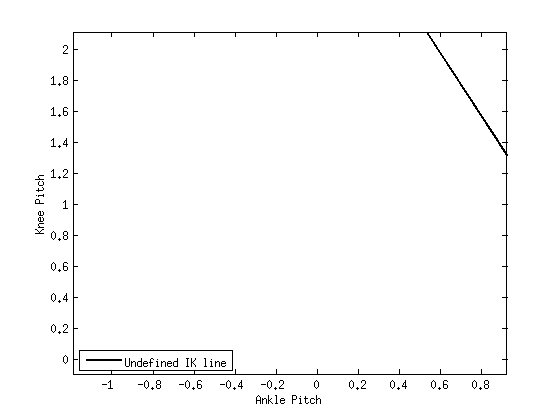
\includegraphics[height = 10cm]{Figures/locus.png}
 		\caption{Undefined Locus For Legs}
 		\label{fig:unlocus}
	\end{center}
\end{figure}

Now we can reconstruct and remove the rotation at the end and the transformation from ankle pitch to ankle roll from the chain to make it simpler
\[
T_{\text{llegRotated}'} = T_\text{llegRotated}\left(T^6_5R_z\left(\pi\right)R_y(-\tfrac{\pi}{2})\right)^{-1}
\]
\[
T_{\text{llegInv}'} = \left( T_{\text{llegRotated}'} \right) ^{-1}
\]
Now we have $p_x = T_{\text{llegInv}'(1,4)}$, $p_y = T_{\text{llegInv}'(2,4)}$ and $p_z = T_{\text{llegInv}'(3,4)}$. From the new symbolic transformation matrix we have:
\begin{align*}
&r_{14} = l_2\cos\theta_5 + l_1\left(\cos\theta_5\cos\theta_4 - \sin\theta_5\sin\theta_4\right)\\
&r_{24} = -l_2\sin\theta_5 - l_1\left(\sin\theta_5\cos\theta_4 + \cos\theta_5\sin\theta_4\right)\\
&r_{34} = 0
\end{align*}
We only need the translation part to extract $\theta_5$, so:
\begin{align*}
&\cos\theta_5\left(l_2+l_1\cos\theta_4\right) = p_x + l_2\sin\theta_5\sin\theta_4 & \Leftrightarrow\\
&\cos\theta_5 = \cfrac{p_x + l_1\sin\theta_5\sin\theta_4}{l_2+l_1\cos\theta_4}&\text{if }l_2+l_1\cos\theta_4\neq0\\
\end{align*}
The $l_2+l_1\cos\theta_4$ is zero if and only if $\cos\theta_4 = 1.029$. So it is always greater than zero, because $-1 \leq \cos \leq 1$:
\begin{align*}
&\sin\theta_5\left(-l_2-l_1\cos\theta_4\right) - l_2\cos\theta_5\sin\theta_4 = p_y& \Leftrightarrow\\
&\sin\theta_5\left(-l_2-l_1\cos\theta_4\right) - l_2\cfrac{p_x + l_1\sin\theta_5\sin\theta_4}{l_2+l_1\cos\theta_4}\sin\theta_4\ =p_y & \Leftrightarrow\\
&-\sin\theta_5\left(l_2+l_1\cos\theta_4\right) - \cfrac{l_2p_x\sin\theta_4}{l_2+l_1\cos\theta_4} - \cfrac{-{l_2}^2\sin\theta_5\sin^2\theta_4}{l_2+l_1\cos\theta_4} = p_y&\Leftrightarrow\\
&-\sin\theta_5\left(l_2+l_1\cos\theta_4\right)^2 - {l_2}^2\sin\theta_5\sin^2\theta_4 = p_y\left(l_2+l_1\cos\theta_4\right) + l_2p_x\sin\theta_4 & \Leftrightarrow\\
&\theta_5 = \arcsin\left(-\frac{p_y\left(l_2+l_1\cos\theta_4\right) + l_1p_x\sin\theta_4}{{l_1}^2\sin^2\theta_4 + \left(l_2 + l_1\cos\theta_4\right)}\right)
\end{align*}
We can do the division because ${l_1}^2\sin^2\theta_4 + \left(l_2 + l_1\cos\theta_4\right)^2$ is obviously greater than zero. 
Now we can remove the two transformations of $\theta_4$ and $\theta_5$ from the symbolic matrix and then we will have a transformation matrix that is a rotation matrix:
\[
T_{\text{llegRotated}''} = T_{\text{llegRotated}'}\left(T^4_3T^5_4\right)^{-1}
\]
\[
T_{\text{llegInv}''} = \left(T_{\text{llegRotated}''}\right)^{-1}
\]
And the rotation part is:
\begin{align*}
&r_{11} = \cos\widehat{\theta}_1\cos\widehat{\theta}_2\cos\theta_4 - \sin\widehat{\theta}_1\sin\theta_3\\
&r_{12} = -\cos\theta_3\sin\widehat{\theta}_1 - \cos\widehat{\theta}_1\cos\widehat{\theta}_2\sin\theta_3\\
&r_{13} = \cos\widehat{\theta}_1\sin\widehat{\theta}_2 \\
&r_{21} = -\cos\theta_3\sin\widehat{\theta}_2\\
&r_{22} = \sin\widehat{\theta}_2\sin\theta_3\\
&r_{23} = \cos\widehat{\theta}_2\\
&r_{31} = -\cos\widehat{\theta}_2\cos\theta_3\sin\widehat{\theta}_1 - \cos\widehat{\theta}_1\sin\theta_3\\
&r_{32} = -\cos\widehat{\theta}_1\cos\theta_3 + \cos\widehat{\theta}_2\sin\widehat{\theta}_1\sin\theta_3\\
&r_{33} = -\sin\widehat{\theta}_1\sin\widehat{\theta}_2
\end{align*}
Finally we can extract, from the transformation matrix, the remaining three angles:
\begin{align*}
\widehat{\theta}_2 &= \arccos T_{\text{llegInv}''(2,3)}\\
\theta_2 &= \widehat{\theta}_2 - \cfrac{\pi}{4}\\
\theta_3 &= \arcsin\left(\cfrac{T_{\text{llegInv}''(2,2)}}{\sin\left(\theta_2+\frac{\pi}{4}\right)}\right)\\
\widehat{\theta}_1 &= \arccos\left(\cfrac{T_{\text{llegInv}''(3,3)}}{\sin\left(\theta_2+\frac{\pi}{4}\right)}\right)\\
\theta_1 &= \widehat{\theta}_1 + \cfrac{\pi}{2}
\end{align*}
The equations above don't have any problem with division by zero because of the restriction of NAO. The HipRoll joint $(\theta_2)$ doesn't reach $-\frac{\pi}{4}$ or $\frac{3\pi}{4}$ so the denominator never becomes zero. Finally, we will do a forward validation step for all possible set of angles.
Below there are all the equations of inverse kinematics for the left leg:
\begin{align*}
T_\text{llegInv} &= \left(R_x(\tfrac{\pi}{4})\left(\left(A^0_\text{Base}\right)^{-1} T_\text{lleg} \left(A^\text{End}_6\right)^{-1}\right)\right)^{-1} \\
\theta_4 &=\pm\left(\pi - \arccos\left(\frac{{l_1}^2 + {l_2}^2 - \sqrt{\left(s_x-p_x\right)^2 + \left(s_y-p_y\right)^2 + \left(s_z-p_z\right)^2}^2}{2 l_1 l_2}\right)\right) \\
\theta_6 &= \arctan\left(\frac{p_y}{p_z}\right)\hspace{3cm}\text{if} \left(l_2\cos\theta_5 + l_1 \cos\left(\theta_4 + \theta_5\right)\right) \neq 0 \\
T_{\text{llegInv}'} &= \left(\left(T_\text{llegInv}\right)^{-1}\left(T^6_5R_z\left(\pi\right)R_y(-\tfrac{\pi}{2})\right)^{-1}\right)^{-1} \\
\theta_5 &= \arcsin\left(-\frac{p_y\left(l_2+l_1\cos\theta_4\right) + l_1p_x\sin\theta_4}{{l_1}^2\sin^2\theta_4 + \left(l_2 + l_1\cos\theta_4\right)}\right) \\
\theta_5 &= \pi - \arcsin\left(-\frac{p_y\left(l_2+l_1\cos\theta_4\right) + l_1p_x\sin\theta_4}{{l_1}^2\sin^2\theta_4 + \left(l_2 + l_1\cos\theta_4\right)}\right)\\
T_{\text{llegInv}''} &= \left(\left(T_{\text{llegInv}'}\right)^{-1}\left(T^4_3T^5_4\right)^{-1}\right)^{-1} \\
\theta_2 &= \pm\arccos T_{\text{llegInv}''(2,3)} - \cfrac{\pi}{4} \\
\theta_3 &= \arcsin\left(\cfrac{T_{\text{llegInv}''(2,2)}}{\sin\left(\theta_2+\frac{\pi}{4}\right)}\right) \\
\theta_3 &= \pi - \arcsin\left(\cfrac{T_{\text{llegInv}''(2,2)}}{\sin\left(\theta_2+\frac{\pi}{4}\right)}\right) \\
\theta_1 &= \pm\arccos\left(\cfrac{T_{\text{llegInv}''(3,3)}}{\sin\left(\theta_2+\frac{\pi}{4}\right)}\right) + \cfrac{\pi}{2}
\end{align*}







\subsection{Inverse Kinematics for the Right Leg}
As we mentioned before, the chains of the legs are symmetric, so we will have a similar solution for the problem as we had with the arms. The only changes are in the rotation matrix that we use to rotate the HipYawPitch joint. Now we must rotate by $-\frac{\pi}{4}$.
\[
T_{\text{rleg}} = A^0_\text{Base}T^1_0T^2_1T^3_2T^4_3T^5_4T^6_5R_z(\pi)R_y(-\tfrac{\pi}{2})A^\text{End}_6
\]
\[
T_{\text{rleg}'} = T_\text{rleg}{\left(A^\text{End}_6\right)}^{-1}
\]
\[
T_{\text{rleg}''} = {\left(A^0_\text{Base}\right)}^{-1}T_{\text{rleg}'}
\]
\[
T_\text{rlegRotated} = R_x(-\tfrac{\pi}{4}) T_{\text{rleg}''}
\]
\[
T_\text{rlegInv} = {\left(T_\text{rlegRotated}\right)}^{-1}
\]
After that, the symbolic matrix for the right leg is exactly the same as the symbolic matrix for the left leg. From this point of view, if we follow all the steps as we did with the left leg, we will conclude to the same equations. So, the final equations are:
\begin{align*}
T_\text{rlegInv} &= \left(R_x(\tfrac{\pi}{4})\left(\left(A^0_\text{Base}\right)^{-1} T_\text{rleg} \left(A^\text{End}_6\right)^{-1}\right)\right)^{-1} \\
\theta_4 &=\pm\left(\pi - \arccos\left(\frac{{l_1}^2 + {l_2}^2 - \sqrt{\left(s_x-p_x\right)^2 + \left(s_y-p_y\right)^2 + \left(s_z-p_z\right)^2}^2}{2 l_1 l_2}\right)\right) \\
\theta_6 &= \arctan\left(\frac{p_y}{p_z}\right)\hspace{3cm}\text{if} \left(l_2\cos\theta_5 + l_1 \cos\left(\theta_4 + \theta_5\right)\right) \neq 0 \\
T_{\text{rlegInv}'} &= \left(\left(T_\text{rlegInv}\right)^{-1}\left(T^6_5R_z\left(\pi\right)R_y(-\tfrac{\pi}{2})\right)^{-1}\right)^{-1} \\
\theta_5 &= \arcsin\left(-\frac{p_y\left(l_2+l_1\cos\theta_4\right) + l_1p_x\sin\theta_4}{{l_1}^2\sin^2\theta_4 + \left(l_2 + l_1\cos\theta_4\right)}\right) \\
\theta_5 &= \pi - \arcsin\left(-\frac{p_y\left(l_2+l_1\cos\theta_4\right) + l_1p_x\sin\theta_4}{{l_1}^2\sin^2\theta_4 + \left(l_2 + l_1\cos\theta_4\right)}\right)\\
T_{\text{rlegInv}''} &= \left(\left(T_{\text{rlegInv}'}\right)^{-1}\left(T^4_3T^5_4\right)^{-1}\right)^{-1} \\
\theta_2 &= \pm\arccos T_{\text{rlegInv}''(2,3)} + \cfrac{\pi}{4} \\
\theta_3 &= \arcsin\left(\cfrac{T_{\text{rlegInv}''(2,2)}}{\sin\left(\theta_2 - \frac{\pi}{4}\right)}\right) \\
\theta_3 &= \pi - \arcsin\left(\cfrac{T_{\text{rlegInv}''(2,2)}}{\sin\left(\theta_2 - \frac{\pi}{4}\right)}\right) \\
\theta_1 &= \pm\arccos\left(\cfrac{T_{\text{rlegInv}''(3,3)}}{\sin\left(\theta_2 - \frac{\pi}{4}\right)}\right) + \cfrac{\pi}{2}
\end{align*}







\subsection{Undefined Target Points For Legs}
\label{undefined}
As we mentioned before, we have some target points for which we can't find an inverse kinematics solution. These target points are presented in the figure~\ref{fig:undefined}, alongside with all the values of the angles that are responsible for this singularity. As we can see, we let the robot to do a lot of movements in the field, and none of those movements was close to the points of the singularity. In real world, it is very rare for someone to give target points in that area. Also, when someone is executing a trajectory, they ''feed'' inverse kinematics with a lot of target points per second (usually they provide inverse kinematics with target points with frequency 50 to 100 Hz), so if one of those target points is in the area of singularity, we will find a solution for the next target point. Because we are working in high frequency rate, the singularity will be unnoticed and the movement will be continued normally.

\begin{figure}[h]
	\begin{center}
		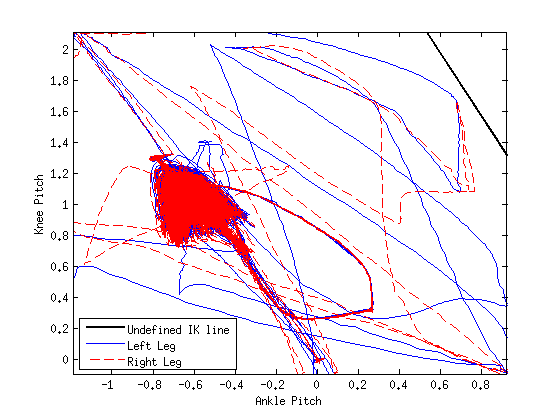
\includegraphics[height = 10cm]{Figures/undefined.png}
 		\caption{Undefined Target Points For Legs}
 		\label{fig:undefined}
	\end{center}
\end{figure}


\section{Implementation}
Now that we have all the equations for both problems, we must integrate them in the code of the team. The code of the team is written in \verb!C++! so because \verb!C++! doesn't have any library for fast linear algebra operations, we must develop a minimalistic matrix framework. Then, using this framework, we must write some functions that will implement the equations of forward and inverse kinematics in \verb!C++!.

\subsection{KMat: Kouretes Math Library}
KMat is a library developed by Emmanouil Orfanoudakis~\cite{orfanoudakis2011} that supports a strict subset of algebraic operations. The focus of the library is mainly in real numbers operations and the primary goal of KMat is low memory footprint and calculation efficiency. The typical linear algebra libraries do run-time validation for the compatibility of the operands and are optimized for large matrices. On the other hand, KMat is optimized for small matrices (typically $(3\times3)$ or $(4\times4)$) and only a subset of operations (addition, subtraction, multiplication, scalar addition, scalar multiplication, transposition, inversion) have been implemented. KMat supports two type of matrices: Dense matrices and Affine transformation matrices.

For our work we used mainly the affine type of matrices and we expanded the functions of the library with some functions that are extremely useful for the kinematics computations. These functions are some initialization functions that initialize a matrix with the given DH parameters or reconstruct of the matrix given the target points etc.

\subsection{Nao Kinematics in C++}
Along with KMat we created two more libraries ForwardKinematics and InverseKinematics. ForwardKinematics has the functions to calculate the location of an end effector of a kinematic chain, given the joint values for this chain. The union of independent chains with common base frame is possible, so someone can take the position of the top camera relatively to one of the legs. Finally, we have a function to calculate the center of mass of the robot. The input of each function is the values of the joints with the order that they appear in the kinematic chains.

The inverse kinematics library has five functions, each of which solves the problem for a kinematic chain. All functions take, as input, the position and the orientation of the target point and the output is the values of the joints, for all the possible solutions for this point. It is possible to have a solution with two set of values and then the user can decide what output will be used. 

As we mentioned before, the legs have one common joint (HipYawPitch) but if we give two target points, one for each leg, inverse kinematics for the left leg will most likely  return a different value for this joint than the inverse kinematics for the right leg. We must decide what value will be set to the HipYawPitch joint and one solution to this problem is to make the support leg (the leg that keeps the robot in balance) the master of this joint or another solution is to get the mean of these two values. Both solutions are not perfect but with a large probability, if we design trajectories carefully, the resulted values from inverse kinematics for this joint will be close enough. Thus, we can use any of these two solutions and the result will be similar to the result if the joint was independent.